\documentclass[tikz,border=8pt]{standalone}
% Shared look for every TikZ diagram. Load with \input{../../tools/tikz-style.tex}
\usepackage[T1]{fontenc}
\usepackage{lmodern}
\renewcommand{\sfdefault}{lmr}  % diagrams use the same serif as the text
\usetikzlibrary{arrows.meta, positioning, shapes.geometric, calc, fit, backgrounds}
\definecolor{cblue}{HTML}{4C78A8}
\definecolor{corange}{HTML}{F58518}
\definecolor{cgreen}{HTML}{54A24B}
\definecolor{cred}{HTML}{E45756}
\definecolor{cpurple}{HTML}{B279A2}
\definecolor{cgrey}{HTML}{6B6B6B}
\tikzset{
  every picture/.style={font=\sffamily, line width=1.2pt},
  box/.style={draw=#1, fill=#1!12, rounded corners=4pt, align=center, inner sep=7pt, minimum height=1.1cm},
  box/.default=cgrey,
  arrow/.style={-{Stealth[length=3mm]}, draw=cgrey, line width=1.4pt},
  title/.style={font=\sffamily\bfseries\Large},
  note/.style={font=\sffamily\small, text=cgrey, align=center},
}
\AtBeginDocument{\hyphenpenalty=10000 \exhyphenpenalty=10000}

\begin{document}
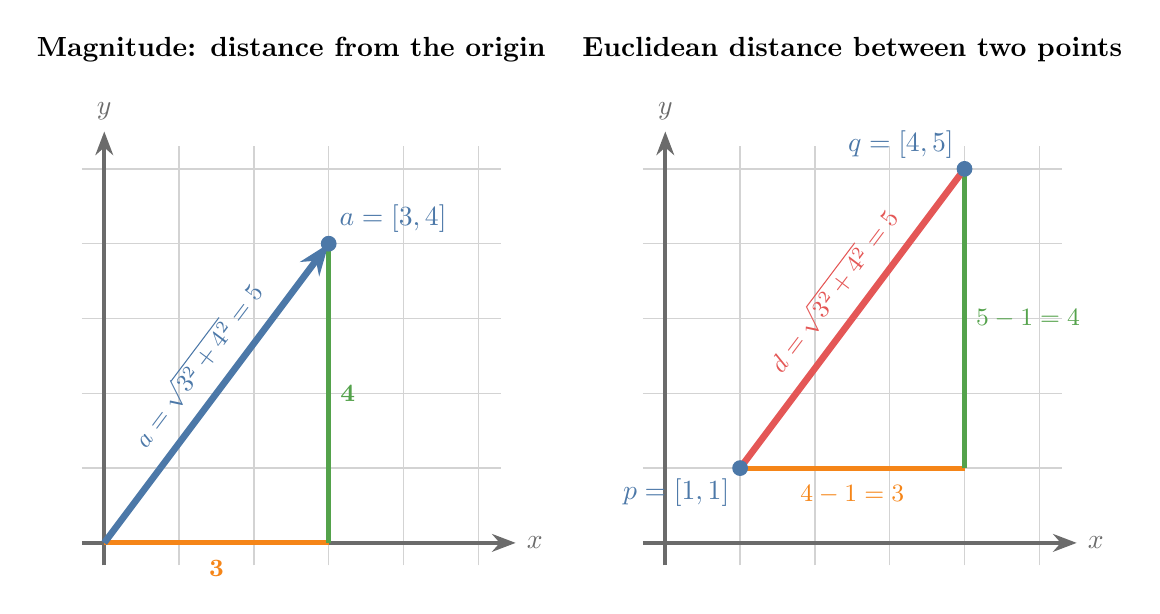
\begin{tikzpicture}[scale=0.95]
  % panel 1: magnitude
  \begin{scope}
    \node[font=\bfseries] at (2.5,6.6) {Magnitude: distance from the origin};
    \draw[cgrey!30, line width=0.5pt] (-0.3,-0.3) grid (5.3,5.3);
    \draw[arrow, cgrey] (-0.3,0) -- (5.5,0) node[right] {$x$};
    \draw[arrow, cgrey] (0,-0.3) -- (0,5.5) node[above] {$y$};
    \draw[corange, line width=1.8pt] (0,0) -- (3,0) node[midway, below=2pt, font=\small\bfseries] {3};
    \draw[cgreen, line width=1.8pt] (3,0) -- (3,4) node[midway, right, font=\small\bfseries] {4};
    \draw[-{Stealth[length=4mm]}, cblue, line width=2.4pt] (0,0) -- (3,4);
    \node[rotate=53, above=5pt, font=\small\bfseries, text=cblue] at (1.5,2) {$\lVert a\rVert = \sqrt{3^2+4^2} = 5$};
    \fill[cblue] (3,4) circle (3pt) node[above right, text=cblue, font=\bfseries] {$a = [3,4]$};
  \end{scope}
  % panel 2: distance
  \begin{scope}[xshift=7.5cm]
    \node[font=\bfseries] at (2.5,6.6) {Euclidean distance between two points};
    \draw[cgrey!30, line width=0.5pt] (-0.3,-0.3) grid (5.3,5.3);
    \draw[arrow, cgrey] (-0.3,0) -- (5.5,0) node[right] {$x$};
    \draw[arrow, cgrey] (0,-0.3) -- (0,5.5) node[above] {$y$};
    \draw[corange, line width=1.8pt] (1,1) -- (4,1) node[midway, below=2pt, font=\small\bfseries] {$4-1=3$};
    \draw[cgreen, line width=1.8pt] (4,1) -- (4,5) node[midway, right, font=\small\bfseries] {$5-1=4$};
    \draw[cred, line width=2.4pt] (1,1) -- (4,5);
    \node[rotate=53, above=5pt, font=\small\bfseries, text=cred] at (2.5,3) {$d = \sqrt{3^2+4^2} = 5$};
    \fill[cblue] (1,1) circle (3pt) node[below left, text=cblue, font=\bfseries] {$p = [1,1]$};
    \fill[cblue] (4,5) circle (3pt) node[above left, text=cblue, font=\bfseries] {$q = [4,5]$};
  \end{scope}
\end{tikzpicture}
\end{document}
